\tool{GnuRadio}

On groundstation PC there's a GNU Radio installed, which is used for both uplink and downlink. In consists of 3 programs (flowcharts):

\begin{itemize}
	\item uplink - waterfall moves only when frame is transmitted, otherwise it's still. All defaults are OK. Closing this windows causes uplink aplikaction shutdown. Example on image \ref{fig:gs:uplink}
	\item funcube_source as interface between FUNCube <-> ZMQ. This application is with GUI. It cannot be openeded twice. Example on image \ref{fig:gs:fcd_source}
	\item downlink that takes data from ZMQ (from funcube_source). All default settings are OK, only Symbol Rate needs manipulation if satellite baudrate has been changed. It needs funcube_source to work properly. Waterfall should be moving all the time. Example on image \ref{fig:gs:downlink}
\end{itemize}

\begin{figure}
	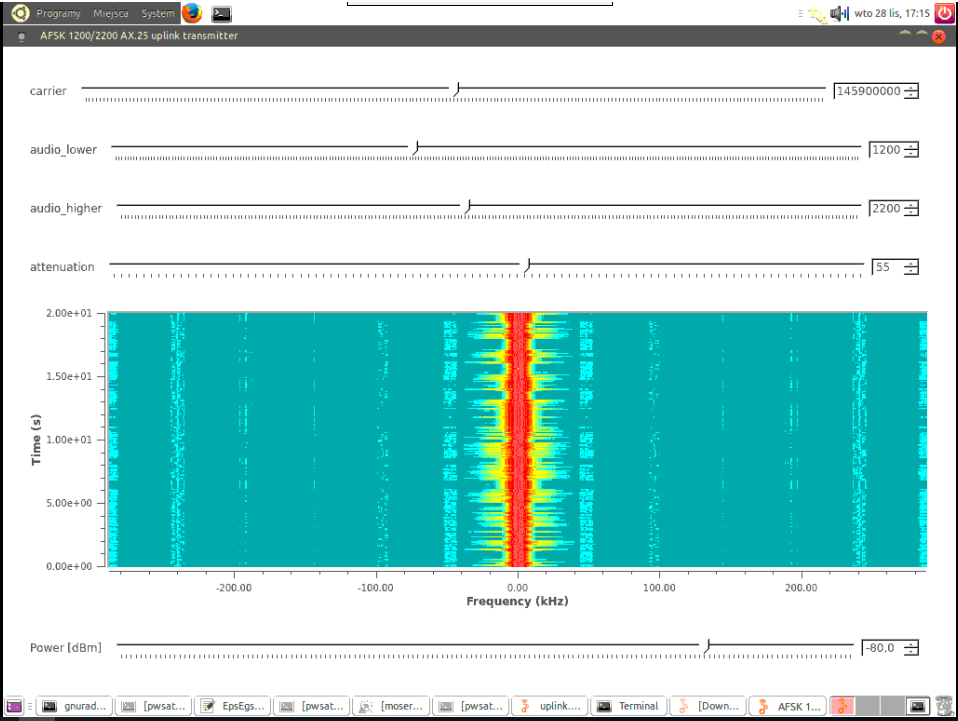
\includegraphics[width=0.8\textwidth]{gs/img/uplink.png}
	\caption{\label{fig:gs:uplink} GNU Radio uplink}
\end{figure}

\begin{figure}
	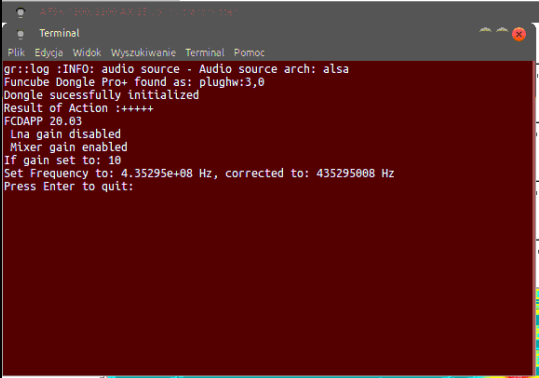
\includegraphics[width=0.8\textwidth]{gs/img/fcd-source.png}
	\caption{\label{fig:gs:fcd_source} FUNcube source}
\end{figure}

\begin{figure}
	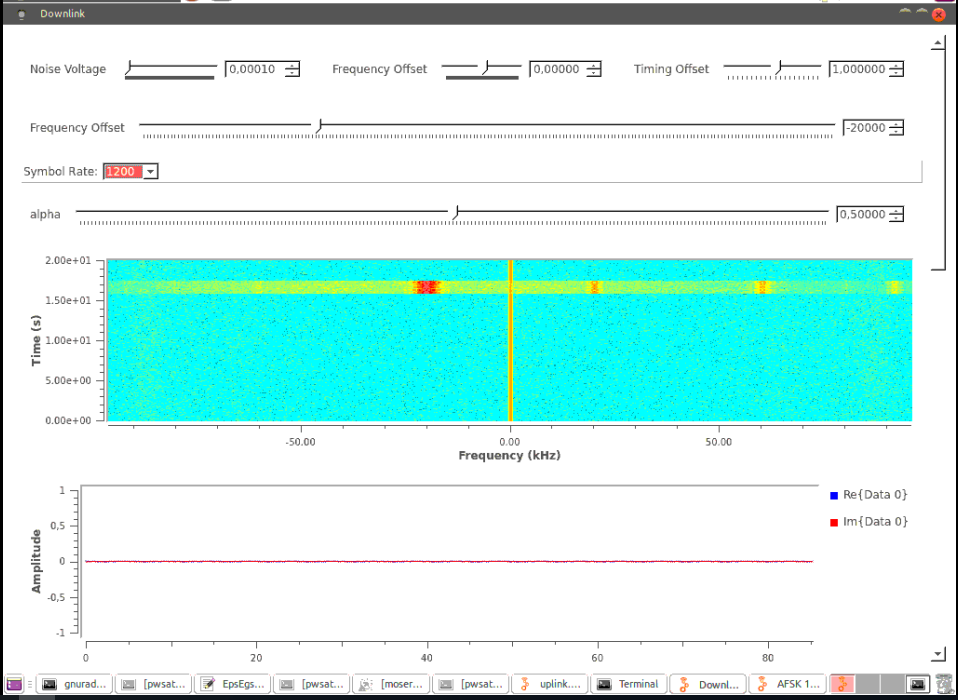
\includegraphics[width=0.8\textwidth]{gs/img/downlink.png}
	\caption{\label{fig:gs:downlink} GNU Radio downlink}
\end{figure}